%%%%%%%%%%%%%%%%%%%%%%%%%%%%%%%%%%%%%%%%%%%%%%%%%%%%%%%%%%%%%%%%%%%%%%%%%%%%%%%%
%2345678901234567890123456789012345678901234567890123456789012345678901234567890
%        1         2         3         4         5         6         7         8

\documentclass[a4paper, 11pt]{article}
\usepackage{comment} % enables the use of multi-line comments (\ifx \fi) 
\usepackage{lipsum} %This package just generates Lorem Ipsum filler text. 
\usepackage{fullpage} % changes the margin
\usepackage{graphicx}
\usepackage{amsmath}
\usepackage{titlesec}
\usepackage{enumitem}
\usepackage{subcaption}
\usepackage{floatrow}%

\title{\LARGE \bf
Question Encoding for Robust QA Networks
}

%\author{ \parbox{3 in}{\centering Huibert Kwakernaak*
%         \thanks{*Use the $\backslash$thanks command to put information here}\\
%         Faculty of Electrical Engineering, Mathematics and Computer Science\\
%         University of Twente\\
%         7500 AE Enschede, The Netherlands\\
%         {\tt\small h.kwakernaak@autsubmit.com}}
%         \hspace*{ 0.5 in}
%         \parbox{3 in}{ \centering Pradeep Misra**
%         \thanks{**The footnote marks may be inserted manually}\\
%        Department of Electrical Engineering \\
%         Wright State University\\
%         Dayton, OH 45435, USA\\
%         {\tt\small pmisra@cs.wright.edu}}
%}

\author{Arnav Vaid$^{1}$, Anaga Rajan$^{2}$, Christopher Correa$^{3}$, and Nikhil Sharma$^{4}$% <-this % stops a space
\thanks{*This work was not supported by any organization}% <-this % stops a space
\thanks{$^{1}$A. Vaid is with the Department of EECS at the UC Berkeley}%
\thanks{$^{2}$A. Rajan is with the Department of EECS at the UC Berkeley}%
\thanks{$^{3}$C. Correa is with the Department of EECS at the UC Berkeley}%
\thanks{$^{4}$N. Sharma is with the Department of EECS at the UC Berkeley}%
}


\begin{document}

\maketitle
\thispagestyle{empty}
\pagestyle{empty}


%%%%%%%%%%%%%%%%%%%%%%%%%%%%%%%%%%%%%%%%%%%%%%%%%%%%%%%%%%%%%%%%%%%%%%%%%%%%%%%%


%%%%%%%%%%%%%%%%%%%%%%%%%%%%%%%%%%%%%%%%%%%%%%%%%%%%%%%%%%%%%%%%%%%%%%%%%%%%%%%%
\section{INTRODUCTION}
There are many ways to syntactically ask the same question. Can we train a machine learning model to map similar questions to a single syntax-invariant representation? We propose using neural techniques to learn a mapping from a typical word-embedding question representation to a syntax-invariant one. \newline\newline
Much progress has been made in learning semantically meaningful representations of words in continuous vector spaces. In this spirit, efforts are being made to learn similar representations for sentences. These embeddings can be learning in an unsupervised manner (techniques like SkipThought [3]), while others can be learned through training for a specific task. \newline\newline
We propose to learn these embeddings by training on sentence similarity tasks. Using a Self-Attentive RNN model [1], we construct an output sequence of new embeddings represented as matrix $M$. We propose an addition to this network which condenses variable length embedding sequences to a single vector representation, which we call the summary vector, allowing explicit comparisons between two questions. We hypothesize that this intermediate embedding sequence $M$ produced by the model will result in a more syntactically invariant representation of a question. \newline\newline
To evaluate the utility of our embeddings, we attempt to use them to train Question-Answering (QA) network. QA networks are tasked with finding the answer to a given question within an article. Good performance on this task requires a good understanding of how syntax affects semantics (Did the cat bite the dog? vs. Did the dog bite the cat?), as well as distilling question meaning in a syntax independent way. We hypothesize that a QA network might converge faster or achieve more robust performance if fed our new embeddings. \newline\newline
We train the Question Encoding network on the Quora Question Pairs dataset, and train the Question Answering network on the Stanford Question Answering Dataset (SQuAD). This should be sufficient data for our purposes; the Quora Question Pairs dataset consists of over 400,000 question pairs and SQuAD is a reading comprehension dataset, consisting of questions posed by crowdworkers on a set of Wikipedia articles containing 10,000+ question-answer pairs on 500+ Wikipedia articles. \newline\newline

\section{APPROACH} 
\subsection{Data Preparation}
In order to first generate our sentence-similarity embeddings, we used a Bidirectional LSTM with self-attention which is typically used for sentence matching tasks [1]. This model was trained on the Quora Question Pairs dataset which contains a series of question pairs and binary label that indicates whether the questions mean the same thing. Then, in order to train our DCN model, both for the baseline and the experimental models, we used the SQuAD (Stanford Question Answering Dataset) which contains a series of questions and reference documents. \newline\newline
Unfortunately, the Quora Question Pairs dataset didn't overlap with the SQuAD dataset and we were unable to find a questions-answers dataset with similar question labels as well, therefore we couldn't perform end-to-end training with our model. Instead, we trained the sentence-embedding model separately, and then used the model when preprocessing the data which was fed into the training process of the DCN.\newline\newline
Furthermore, we used the 300-dimension, Global Vectors for Words Representation (GloVe) to embed our sentences throughout the project, in both the Sentence-Similarity model and the DCN. 

\subsection{Baseline Model}
Our baseline Dynamic Coattention model is already the current state-of-the-art question answering model [2], shown in Figure \ref{fig:dcn}. The model has co-dependent modules that encode the question and document. Then, the outputs are given to the co-attention module that iteratively makes improvements to a dynamic pointer that narrows down on the relevant parts of the reference text. The paper reports that the model achieves a 75.9 F1 score on the SQuAD dataset.  When we train the DCN model, we achieve approximately a 62 F1 score.  

\begin{figure}[h!]
  \center
  \includegraphics[width=12cm]{baseline.png}
  \caption{Dynamic Pointer Decoder}
\end{figure}

\begin{figure}[h!]
  \center
  \includegraphics[width=12cm]{dcn.png}
  \caption{DCN Model Architecture}
  \label{fig:dcn}
\end{figure}

\subsection{Question Encoding Network}
Our QE Network uses an architecture described in [1] consisting of an LSTM that generates a sequence of hidden states, consolidated as a matrix $H$. Self-attention is computed using a feed-forward network to produce matrix $A$, which is then multiplied by $H$ to produce $M$, the sentence embedding. The architecture is visualized in Figure \ref{fig:question_embeddings}. 

\begin{equation}
\begin{split}
H & = (h_1,h_2,\dots,h_n) \\
A & = softmax(W_{s2}tanh(W_{s1}H^T) \\
M & = AH
\end{split}
\end{equation}

\begin{figure}[h!]
  \center
  \includegraphics[width=10cm]{question_embedding.png}
  \caption{Sentence Embedding Architecture}
  \label{fig:question_embeddings}
\end{figure}

Given our training data consists of question pairs, our network needs to generate an sequence-length invariant representation of the questions. We propose to do this by computing vanilla attention over the columns of the sentence embedding $M$ to get the 'summary vector' $m$ as shown in Figure \ref{fig:QE_Arch}. We use an L1 similarity metric as input to a binary cross-entropy loss function to train our network. By training on the task of identifying similar questions, we hypothesize that the $M$ matrix will learn a syntax invariant representation of the question, and $m$ will capture the semantic meaning of a question.

\subsection{Final Model} \label{final_model}

The goal for the final model was to utilize the sentence-similarity representations from the Bi-directional LSTM to create a semantics-free representation that could be used to improve the performance of the DCN. The high-level idea is portrayed in Figure \ref{fig:DCN_QE}. Ideally, the first model would strip away the syntax variations between similar questions and leave behind a representation that only carried the meaning of the question.  We have attempted several methods to incorporate this representation in the DCN inputs.
\begin{enumerate}[label=(\alph*)]
\item In our initial model, we decided to integrate the sentence-embeddings by first training the Bidirectional LSTM. Then, when training our DCN model, instead of passing in the questions directly, we first run it through our sentence-embedding model and then use the $M$ matrix embedding as our question. This $M$ matrix is a series of weighted sums over the hidden states in the LSTM model. In practice, we believed that the columns of $M$ encoded the meaning of the sentence in a syntax-free manner. 

\item Our belief is that the the DCN was unable to train adequately because the second attention over the columns of $M$ might mean the column orderings would not be prioritized in the Question Encoding Network loss function, but would be necessary for the DCN model. Therefore we decided to input to the DCN the original GloVe embeddings, but append the summary vector $m$ to the end of the sequence. We believed this would get rid of the problem of column ordering affecting the network. 

\item This again didn't produce as well of a result as we wanted, as our performance stayed pretty similar to the baseline. Our next iteration carried two major changes: (1) We reverted back to the $M$-matrix and appended it to the glove-embedded question and (2) Used two separate LSTMs in the DCN to train the document and question (due to differing input dim sizes). 

\item After this trial, we decided to take a closer look at what our Bidirectional LSTM was attending to, in hopes of figuring out why our DCN wasn't able use the embeddings to decipher the question. We used an attention-visualizer and found that the model was significantly attending to the padding around $H$, the aggregate of our hidden states. This padding was intended only to bring all queries to the same length and encoded no information. Therefore in our final iteration, we masked the attention over the padding. We additionally reverted back to using our summary vector appended to our question similar to the second model but kept the separated LSTM architecture from the third model.
\end{enumerate}

\begin{figure}[h!]
  \center
  \includegraphics[width=12cm]{QE_Network.png}
  \caption{Question Answering Network Architecture}
  \label{fig:QE_Arch}
\end{figure}

\begin{figure}[h!]
  \center
  \includegraphics[width=12cm]{img3.png}
  \caption{DCN with Question Encoding Network as input}
  \label{fig:DCN_QE}
\end{figure}

% \section{END GOALS}

% In this experiment we hope to improve on the current, state-of-the-art Dynamic Coattention Network (DCN) model for question answering tasks. As per our hypothesis, we believe that incorporating the sentence-similarity embedding to the input of our DCN will improve its performance by bolstering its ability to ignore semantic variance. 

\section{RESULTS}

\begin{figure}[!h]
\begin{floatrow}
\ffigbox{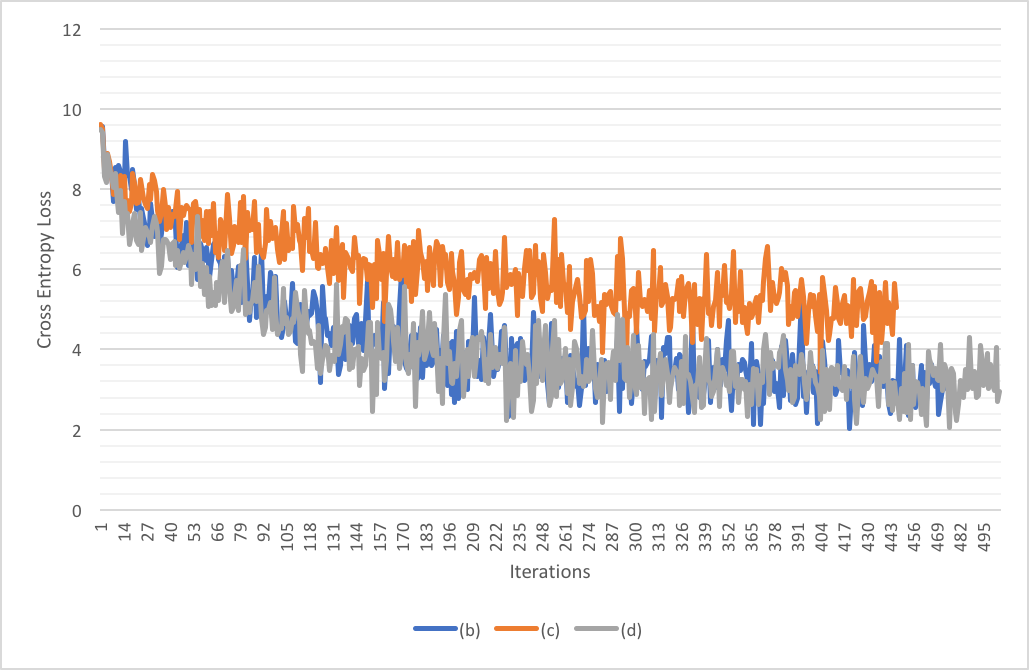
\includegraphics[width=.97\linewidth]{QE_TR_CROSS_ENTROPY_LOSS.png}}{\caption{QE Net Cross Entropy Loss}\label{fig:train_f1}}
\ffigbox{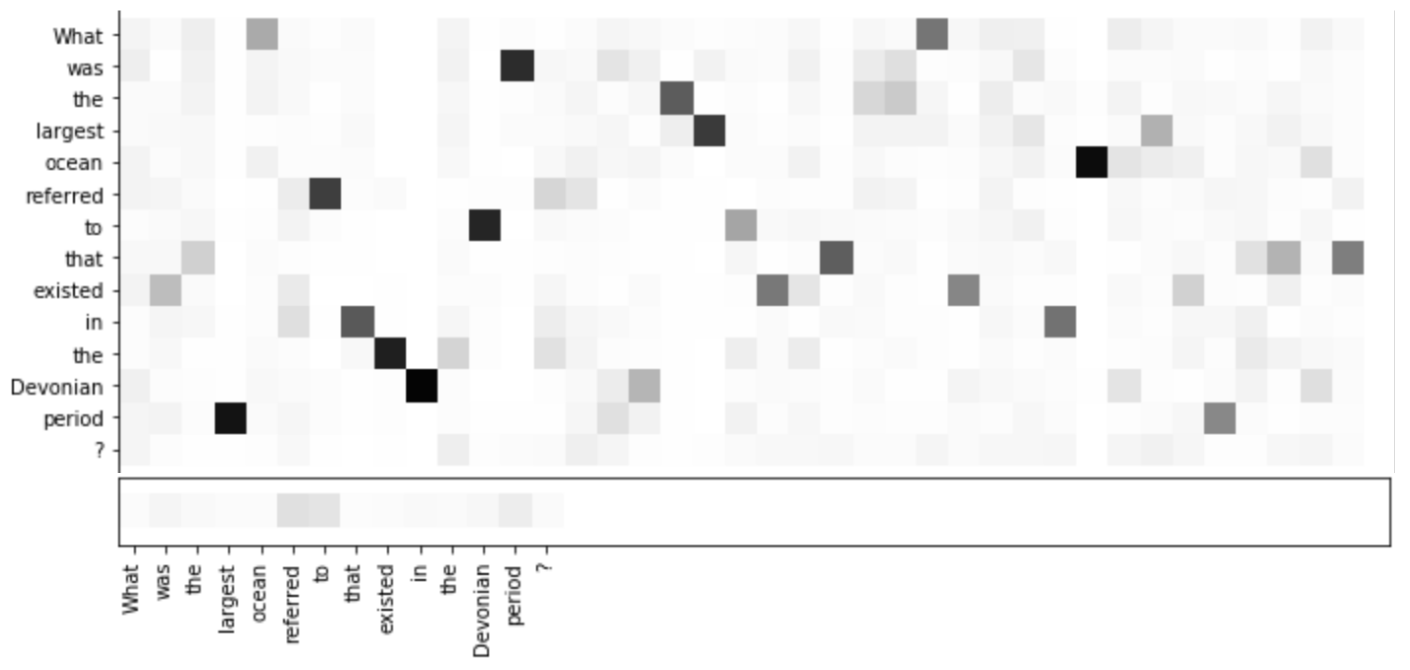
\includegraphics[width=.97\linewidth]{AttentionMap.png}}{\caption{Attention Maps for $A$ Matrix (above) and Vector $a$(below)}\label{fig:val_f1}}
\end{floatrow}
\end{figure}

\begin{figure}
	\centering
      \begin{subfigure}{.5\textwidth}
        \centering
        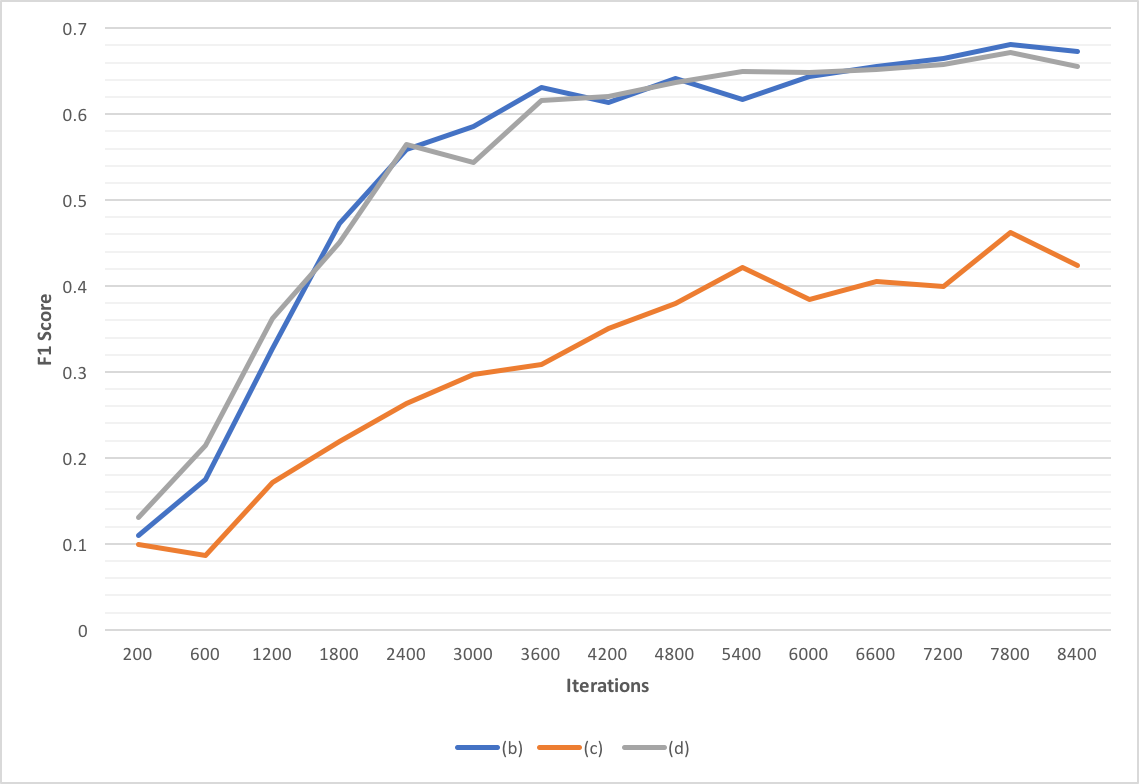
\includegraphics[width=.97\linewidth]{DCN_TR_F1.png}
        \caption{Training F1 Score}
        \label{fig:train_f1}
      \end{subfigure}%
      \begin{subfigure}{.5\textwidth}
        \centering
        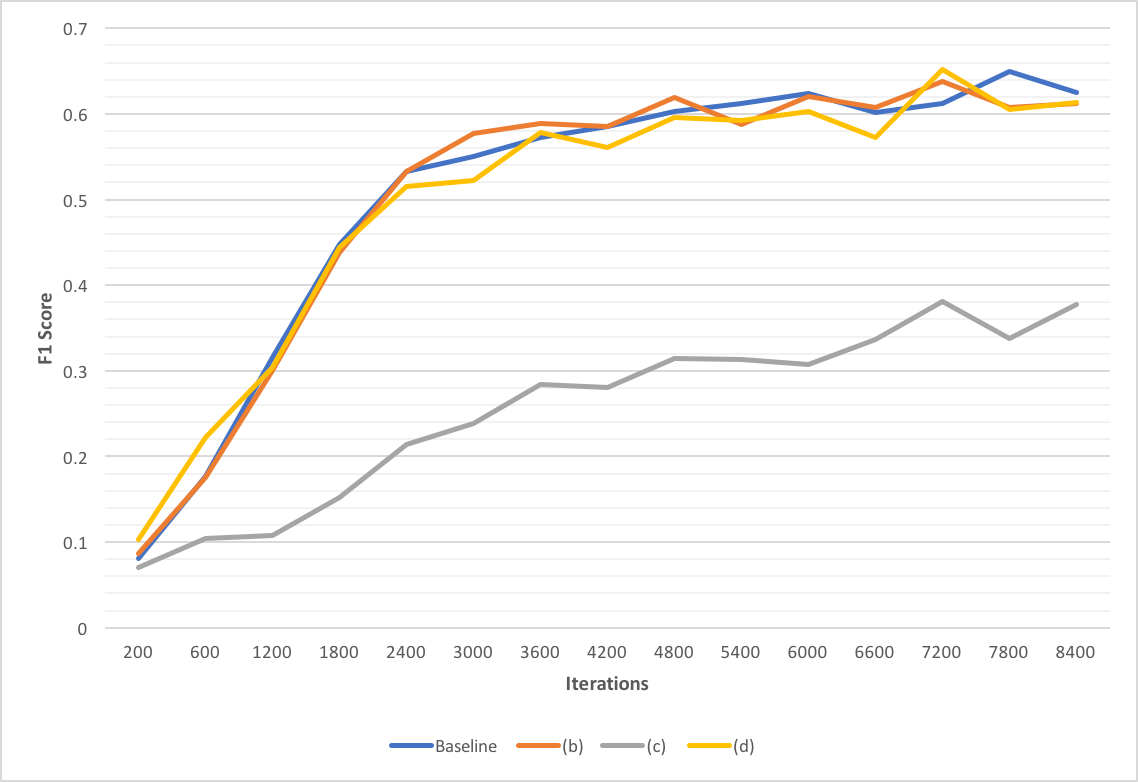
\includegraphics[width=.94\linewidth]{DCN_VAL_F1+Baseline.png}
        \caption{Validation F1 Score}
        \label{fig:val_f1}
      \end{subfigure}
      \caption{F1 Scores for Models in Section \ref{final_model}}
      \label{fig:test}
\end{figure}

We found that simply training the DCN on just the question embeddings led to the model performing very poorly.  We identify two potential reasons for this.  We believe the learned question embeddings are well suited for characterizing the sentence into a summery, but individually do not retain the word relationships that GloVe encodes.  Second, we believe of the second attention module, the columns of $M$ of similar questions don’t need to be in the same order to be classified as the same, but should be in the same order for the question answering network.  The modifications to include the Question Encoded Summary Vector was able to achieve comparable performance to the baseline, but was not able to significantly beat the baseline.  Modifications such as the separate LSTMs for the Question and Document and masking the Attention were not able to help increase performance.  

\section{TOOLS}
This project borrowed from Github repos containing existing frameworks for processing the Quora Question Pairs Dataset, Siamese BiLSTM architecture for the Question Encoding Network, as well as the DCN for our baseline QA Network. Tensorflow was used due to its mature library of functions and because our group was most familiar with it. Pandas, NLTK, and Matplotlib were used for preprocessing and visualization. We used the AWS AMI instance for quite training of our networks.

\section{LESSONS LEARNED}
The biggest hindrance to gaining working results was the time taken to train the models. The Question Encoding Network and DCN took $\sim$4 hours and $\sim$8 hours respectively to reach saturation. As a consequence the design iteration time was slow, and hyperparameter searches were difficult to do. \newline\newline 
Additionally, while borrowing implementations off Github eased the initial burden of writing preprocessing and training pipelines from scratch, it was also a pain to integrate repos, especially when it came to importing models. As a result we resorted to messy hacks that were not the best way to design the project. \newline\newline
Both models also used different data sources with different vocabularies which was hard to coalesce together, for we didn't have any end-to-end datasets which could be used to test our entire model and validate efficiently. \newline\newline
Finally, we learned that attention on variable length sequences mixed with contrastive-style loss can be tricky since attention weights can be learned that correspond to meaningless padding vectors. Future avenues of research would be to utilize transformer networks, which contain multi-headed attention modules that could be more expressive that our model. 

\subsection{Future Work}
It is our hope that our ability to match the baseline results shows significant promise, and that additional hyperparameter tuning and minor modeling assumptions under our defined syntax-invariant paradigm will allow our model to exceed the current state-of-the-art result for Question Answering.

\section{TEAM CONTRIBUTIONS}
\begin{enumerate}
	\item \textbf{Christopher Correa}: Built QE Network, Integrated and Modified DCN, Wrote Report, Handled AWS training.  40\%
    \item \textbf{Arnav Vaid}: Built QE Network, Integrated and Modified DCN, Wrote Visualizations, Wrote Report. 40\%
    \item \textbf{Anaga Rajan}: AWS training, contrastive loss, Wrote Report.  15\%
    \item \textbf{Nikhil Sharma}: Wrote Report.  5\%
\end{enumerate}


\addtolength{\textheight}{-12cm}   % This command serves to balance the column lengths
                                  % on the last page of the document manually. It shortens
                                  % the textheight of the last page by a suitable amount.
                                  % This command does not take effect until the next page
                                  % so it should come on the page before the last. Make
                                  % sure that you do not shorten the textheight too much.

%%%%%%%%%%%%%%%%%%%%%%%%%%%%%%%%%%%%%%%%%%%%%%%%%%%%%%%%%%%%%%%%%%%%%%%%%%%%%%%%



%%%%%%%%%%%%%%%%%%%%%%%%%%%%%%%%%%%%%%%%%%%%%%%%%%%%%%%%%%%%%%%%%%%%%%%%%%%%%%%%



%%%%%%%%%%%%%%%%%%%%%%%%%%%%%%%%%%%%%%%%%%%%%%%%%%%%%%%%%%%%%%%%%%%%%%%%%%%%%%%%

\begin{thebibliography}{99}

\bibitem{c1}Zhouhan Lin, Minwei Feng, Cicero Nogueira dos Santos, Mo Yu, 
      Bing Xiang, Bowen Zhou, and Yoshua Bengio. A structured 
      self-attentive sentence embedding. arXiv preprint 
      arXiv:1703.03130, 2017
\bibitem{c2}Caiming Xiong, Victor Zhong, and Richard Socher. 2016.  
      Dynamic coattention networks for question answering.  arXiv 
      preprint arXiv:1611.01604.
\bibitem{c3} Ryan Kiros, Yukun Zhu, Ruslan R Salakhutdinov, Richard Zemel, 
      Raquel Urtasun, Antonio Torralba, and Sanja Fidler. 
      Skip-thought vectors. In NIPS, 2015.




\end{thebibliography}




\end{document}